\documentclass[11pt]{article}
\usepackage[pdftex]{graphicx}
\usepackage[explicit]{titlesec}
\usepackage[OT1]{fontenc}
\usepackage[most]{tcolorbox}
\usepackage[final]{pdfpages}
\usepackage[colorlinks=true, urlcolor=cyan, hyperfootnotes=false]{hyperref}
\usepackage{fullpage, graphicx, psfrag, url, caption, authblk, amsfonts, amsmath, amssymb, float, fancyhdr, multicol, cmbright, xcolor, amsthm, gensymb, physics}

\fancypagestyle{pages}{
	%Headers
	\fancyhead[L]{Physics 7A, Summer 2024 \\ Section 103}
	%\fancyhead[C]{\thepage}
	\fancyhead[R]{Discussion 2 \\ June 18}
\renewcommand{\headrulewidth}{0pt}
	%Footers
	%\fancyfoot[L]{}
	\fancyfoot[C]{}
	\fancyfoot[R]{\thepage}
\renewcommand{\footrulewidth}{0pt}
}

\newcommand\blfootnote[1]{
    \begingroup
    \renewcommand\thefootnote{}\footnote{#1}
    \addtocounter{footnote}{-1}
    \endgroup
}

\newcommand{\fig}[4]{
    \begin{figure}[H]
        \centering
        \includegraphics[scale={#3}, angle={#4}]{#1}
        \caption{#2}
        \label{exp4fit}
    \end{figure}
}

\newtheoremstyle{gangnamstyle}{}{}{}{}{\sffamily\bfseries}{.}{ }{}
\tcolorboxenvironment{definition}{boxrule=0pt,boxsep=0pt,colback={blue!10},left=8pt,right=8pt,enhanced jigsaw, borderline west={2pt}{0pt}{blue},sharp corners,before skip=10pt,after skip=10pt,breakable}
\tcolorboxenvironment{example}{boxrule=0pt,boxsep=0pt,colback={orange!10},left=8pt,right=8pt,enhanced jigsaw, borderline west={2pt}{0pt}{orange},sharp corners,before skip=10pt,after skip=10pt,breakable}
\tcolorboxenvironment{problem}{boxrule=0pt,boxsep=0pt,colback={cyan!10},left=8pt,right=8pt,enhanced jigsaw, borderline west={2pt}{0pt}{cyan},sharp corners,before skip=10pt,after skip=10pt,breakable}
\theoremstyle{gangnamstyle}{\newtheorem{definition}{Definition}[]}
\theoremstyle{gangnamstyle}{\newtheorem{example}{Example}[]}
\theoremstyle{gangnamstyle}{\newtheorem{problem}{Problem}[]}

\headheight=0pt
\footskip=0pt
\setlength{\oddsidemargin}{0 in}
\setlength{\evensidemargin}{0 in}
\setlength{\topmargin}{-0.5 in}
\setlength{\textwidth}{6.5 in}
\setlength{\textheight}{8.5 in}
\setlength{\headsep}{0.75 in}
\setlength{\parindent}{0 in}
\setlength{\parskip}{0.1 in}

\begin{document}
\normalfont
\pagestyle{pages}

% Begin Document

\begin{center}
\vspace{3in}
{\Large Discussion 2 } \\ [0.05in]
1D Kinematics \\ [-0.5in]
\end{center}

\section*{Topics}
Position, Velocity, and Acceleration; Formulas for Constant Acceleration

\section{Review}

\begin{itemize}
\item For a function $f(x)$, its derivative $\frac{df}{dx}$ is the slope on the $f$ vs $x$ graph. Its integral $\int f(x) \ dx$ is the area enclosed between $f$ and the $x$-axis. 

\item Average value of a function. Let $f(x)$ be a function, and $F(x) = \int f(x) \ dx$ be its integral. \\
The average value of $f$ between $a \leq x \leq b$ is
\[ f_{avg} = \frac{1}{b - a} \int_a^b f(x) \ dx = \frac{F(b) - F(a)}{b - a} \]

\item Velocity \textcolor{blue}{(Acceleration)} is the derivative of Position \textcolor{blue}{(Velocity)}. 
\[ v = \frac{dx}{dt} \]
\[ a = \frac{dv}{dt} \]
Position \textcolor{blue}{(Velocity)} is the integral of Velocity \textcolor{blue}{(Acceleration)}. 
\[ x = x_0 + \int_0^t v \ dt \]
\[ v = v_0 + \int_0^t a \ dt \]

\item All objects at the surface of the Earth experience a constant downward acceleration of 
\[ g = 9.8 m/s^2 \]

\item If an object moves in a straight line with \textbf{Constant Acceleration} $a$, the formulas below can be applied. 
\[ v = v_0 + at \]
\[ x = x_0 + v_0t + \frac{1}{2}at^2 \]
\[ v^2 = v_0^2 + 2a(x - x_0) \]
\[ v_{avg} = \frac{1}{2}(v + v_0) \]
The subscript $0$ denotes an initial value at $t = 0$. Variables without subscripts denote quantities at time $t$. 
\end{itemize}

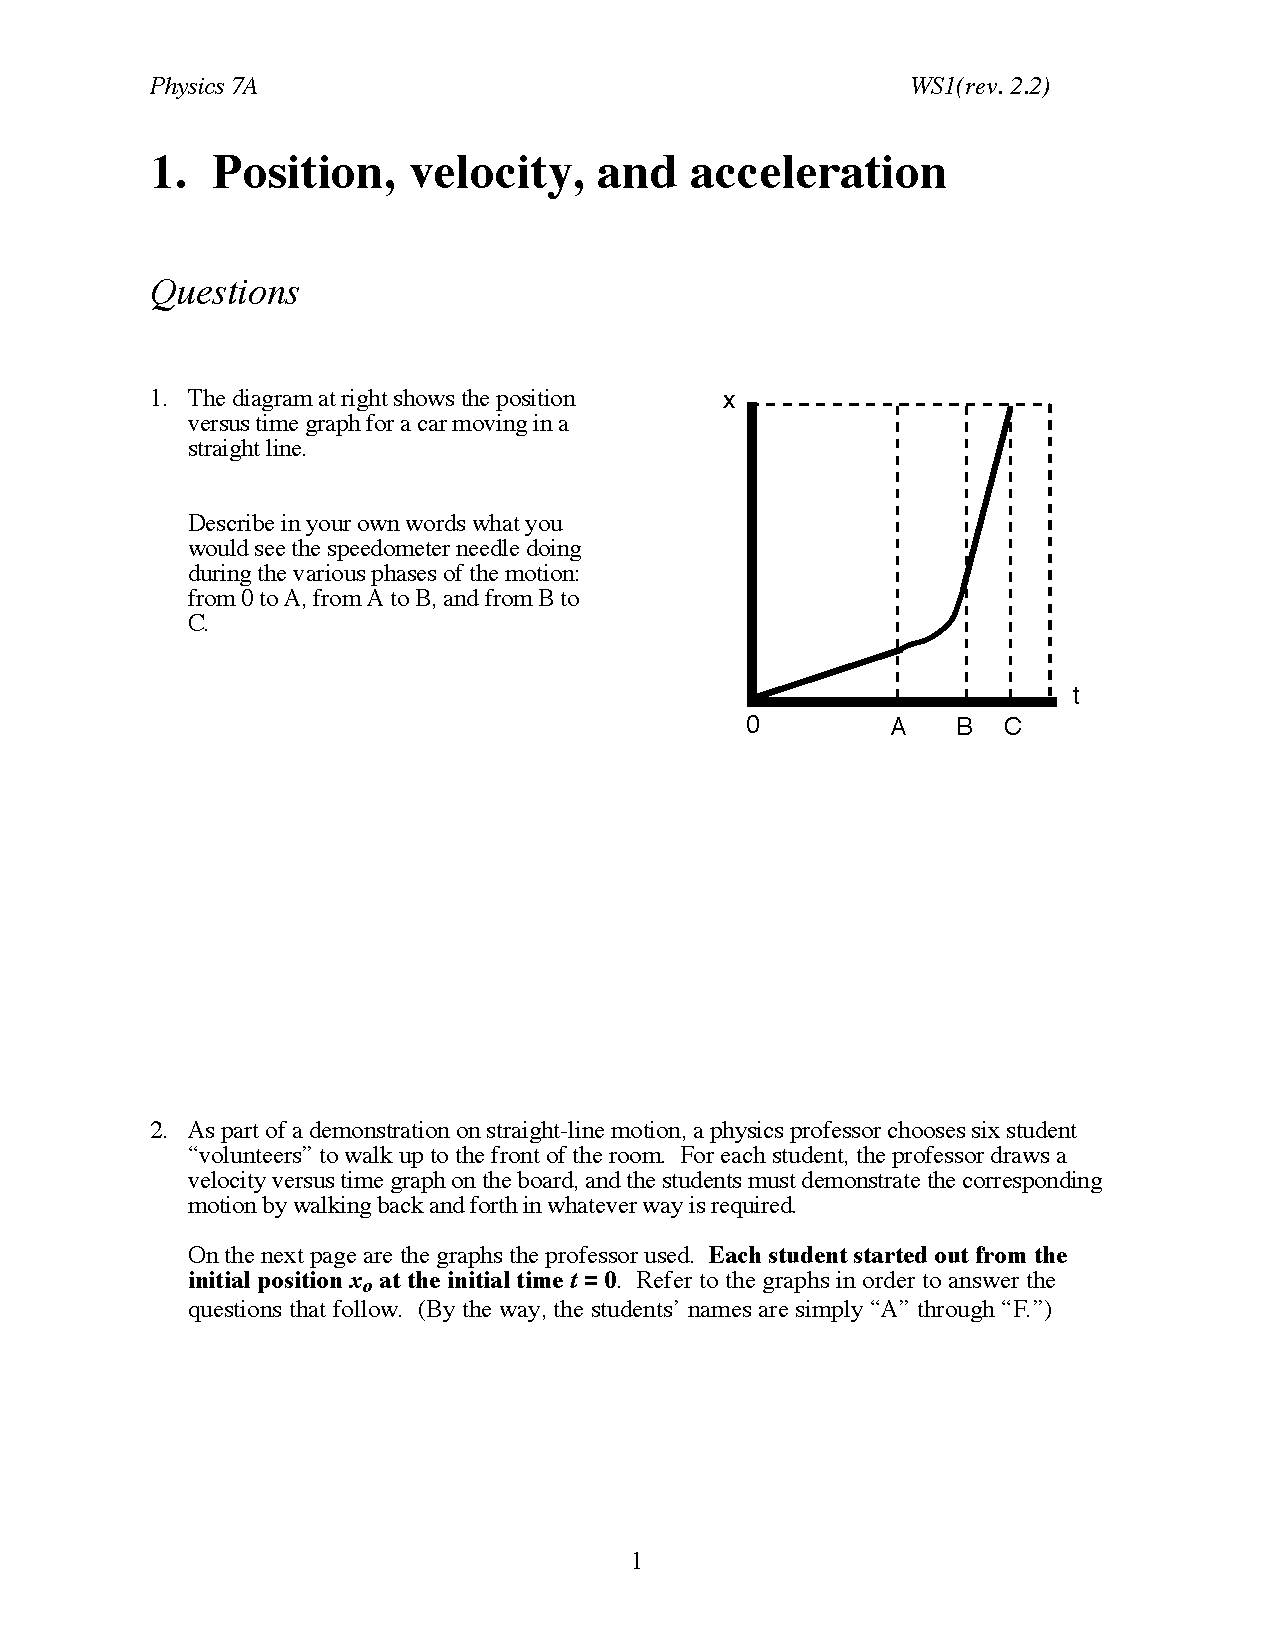
\includepdf[pages=-]{figs/0618/ws1.pdf}

\end{document}
